\documentclass[a4paper,landscape,final,8pt]{beamer} % Tamaño de papel, tamaño de letra y clase LaTeX usada. Otras clases: book, beamer...
\usepackage[spanish]{babel}
\usepackage[utf8]{inputenc}
\usepackage[T1]{fontenc} % Permite cambiar la fuente por defecto.
\usepackage{anysize}     % Permite modificar el tamaño de los márgenes.
\usepackage{multicol}    % Permite escribir a doble, triple...columna.
\usepackage{graphicx}    % Permite implementar imágenes.
\usepackage{multirow}        % Para fusionar filas
\usepackage{helvet}
\usepackage{colortbl}
\usepackage{hhline}

\usepackage[absolute,overlay]{textpos}
\setlength{\TPHorizModule}{1cm}
\setlength{\TPVertModule}{1cm}


\renewcommand{\familydefault}{\sfdefault}

%ORDENES PARA PERSONALIZAR EL FORMATO DE TU DOCUMENTO
\marginsize{1.5cm}{1cm}{0.5cm}{1.5cm} % MÁRGENES: Izq, Der, Sup, Inf.
\parindent=0mm                        % Sangría por defecto.
\parskip=3mm                          % Espacio entre párrafos por defecto.
\renewcommand{\baselinestretch}{1}    % Interlineado.
\definecolor{00E500}{HTML}{00E500}
\definecolor{FFFE25}{HTML}{FFFE25}
\definecolor{FF0000}{HTML}{FF0000}

\begin{document}   % Orden que marca el inicio del artículo.

\usebackgroundtemplate{%
  
\includegraphics[width=0.98\paperwidth,height=0.98\paperheight]{./Images/Background.pdf}%
}


\expandafter\def\csname HELOa06a1aC\endcsname{00E500}
\expandafter\def\csname HELOa06a1aT\endcsname{}
\expandafter\def\csname STOVLa06a1aC\endcsname{00E500}
\expandafter\def\csname STOVLa06a1aT\endcsname{}
\expandafter\def\csname VEHICLESa06a1aC\endcsname{00E500}
\expandafter\def\csname VEHICLESa06a1aT\endcsname{}
\expandafter\def\csname PERSONNELa06a1aC\endcsname{00E500}
\expandafter\def\csname PERSONNELa06a1aT\endcsname{}
\expandafter\def\csname SCATa06a1aC\endcsname{FFFE25}
\expandafter\def\csname SCATa06a1aT\endcsname{SS, N}
\expandafter\def\csname LNDa06a1aC\endcsname{FF0000}
\expandafter\def\csname LNDa06a1aT\endcsname{SS}
\expandafter\def\csname RHIBa06a1aC\endcsname{FFFE25}
\expandafter\def\csname RHIBa06a1aT\endcsname{SS, N}
\expandafter\def\csname RASFASa06a1aC\endcsname{FFFE25}
\expandafter\def\csname RASFASa06a1aT\endcsname{SS, N}
\expandafter\def\csname AAWa06a1aC\endcsname{00E500}
\expandafter\def\csname AAWa06a1aT\endcsname{}
\expandafter\def\csname ASWa06a1aC\endcsname{00E500}
\expandafter\def\csname ASWa06a1aT\endcsname{}
\expandafter\def\csname ASUWa06a1aC\endcsname{FFFE25}
\expandafter\def\csname ASUWa06a1aT\endcsname{P}
\expandafter\def\csname HELOa12aC\endcsname{FFFE25}
\expandafter\def\csname HELOa12aT\endcsname{SS}
\expandafter\def\csname STOVLa12aC\endcsname{FFFE25}
\expandafter\def\csname STOVLa12aT\endcsname{SS}
\expandafter\def\csname VEHICLESa12aC\endcsname{00E500}
\expandafter\def\csname VEHICLESa12aT\endcsname{}
\expandafter\def\csname PERSONNELa12aC\endcsname{FFFE25}
\expandafter\def\csname PERSONNELa12aT\endcsname{SS}
\expandafter\def\csname SCATa12aC\endcsname{FF0000}
\expandafter\def\csname SCATa12aT\endcsname{W, SS}
\expandafter\def\csname LNDa12aC\endcsname{FF0000}
\expandafter\def\csname LNDa12aT\endcsname{SS}
\expandafter\def\csname RHIBa12aC\endcsname{FF0000}
\expandafter\def\csname RHIBa12aT\endcsname{W, SS}
\expandafter\def\csname RASFASa12aC\endcsname{FF0000}
\expandafter\def\csname RASFASa12aT\endcsname{W, SS}
\expandafter\def\csname AAWa12aC\endcsname{00E500}
\expandafter\def\csname AAWa12aT\endcsname{}
\expandafter\def\csname ASWa12aC\endcsname{FFFE25}
\expandafter\def\csname ASWa12aT\endcsname{SS}
\expandafter\def\csname ASUWa12aC\endcsname{FFFE25}
\expandafter\def\csname ASUWa12aT\endcsname{SS, P}
\expandafter\def\csname HELOa18aC\endcsname{FFFE25}
\expandafter\def\csname HELOa18aT\endcsname{SS}
\expandafter\def\csname STOVLa18aC\endcsname{FFFE25}
\expandafter\def\csname STOVLa18aT\endcsname{SS}
\expandafter\def\csname VEHICLESa18aC\endcsname{00E500}
\expandafter\def\csname VEHICLESa18aT\endcsname{}
\expandafter\def\csname PERSONNELa18aC\endcsname{FFFE25}
\expandafter\def\csname PERSONNELa18aT\endcsname{SS}
\expandafter\def\csname SCATa18aC\endcsname{FF0000}
\expandafter\def\csname SCATa18aT\endcsname{SS}
\expandafter\def\csname LNDa18aC\endcsname{FF0000}
\expandafter\def\csname LNDa18aT\endcsname{SS}
\expandafter\def\csname RHIBa18aC\endcsname{FF0000}
\expandafter\def\csname RHIBa18aT\endcsname{SS}
\expandafter\def\csname RASFASa18aC\endcsname{FF0000}
\expandafter\def\csname RASFASa18aT\endcsname{SS}
\expandafter\def\csname AAWa18aC\endcsname{00E500}
\expandafter\def\csname AAWa18aT\endcsname{}
\expandafter\def\csname ASWa18aC\endcsname{FFFE25}
\expandafter\def\csname ASWa18aT\endcsname{SS}
\expandafter\def\csname ASUWa18aC\endcsname{FFFE25}
\expandafter\def\csname ASUWa18aT\endcsname{SS, P}
\expandafter\def\csname HELOa00aC\endcsname{FFFE25}
\expandafter\def\csname HELOa00aT\endcsname{SS}
\expandafter\def\csname STOVLa00aC\endcsname{FFFE25}
\expandafter\def\csname STOVLa00aT\endcsname{SS}
\expandafter\def\csname VEHICLESa00aC\endcsname{00E500}
\expandafter\def\csname VEHICLESa00aT\endcsname{}
\expandafter\def\csname PERSONNELa00aC\endcsname{FFFE25}
\expandafter\def\csname PERSONNELa00aT\endcsname{SS}
\expandafter\def\csname SCATa00aC\endcsname{FF0000}
\expandafter\def\csname SCATa00aT\endcsname{W, SS, N}
\expandafter\def\csname LNDa00aC\endcsname{FF0000}
\expandafter\def\csname LNDa00aT\endcsname{SS}
\expandafter\def\csname RHIBa00aC\endcsname{FF0000}
\expandafter\def\csname RHIBa00aT\endcsname{W, SS, N}
\expandafter\def\csname RASFASa00aC\endcsname{FF0000}
\expandafter\def\csname RASFASa00aT\endcsname{W, SS, N}
\expandafter\def\csname AAWa00aC\endcsname{00E500}
\expandafter\def\csname AAWa00aT\endcsname{}
\expandafter\def\csname ASWa00aC\endcsname{FFFE25}
\expandafter\def\csname ASWa00aT\endcsname{SS}
\expandafter\def\csname ASUWa00aC\endcsname{FFFE25}
\expandafter\def\csname ASUWa00aT\endcsname{SS, P}
\expandafter\def\csname HELOa06a2aC\endcsname{00E500}
\expandafter\def\csname HELOa06a2aT\endcsname{}
\expandafter\def\csname STOVLa06a2aC\endcsname{00E500}
\expandafter\def\csname STOVLa06a2aT\endcsname{}
\expandafter\def\csname VEHICLESa06a2aC\endcsname{00E500}
\expandafter\def\csname VEHICLESa06a2aT\endcsname{}
\expandafter\def\csname PERSONNELa06a2aC\endcsname{00E500}
\expandafter\def\csname PERSONNELa06a2aT\endcsname{}
\expandafter\def\csname SCATa06a2aC\endcsname{FFFE25}
\expandafter\def\csname SCATa06a2aT\endcsname{SS, N}
\expandafter\def\csname LNDa06a2aC\endcsname{FF0000}
\expandafter\def\csname LNDa06a2aT\endcsname{SS}
\expandafter\def\csname RHIBa06a2aC\endcsname{FFFE25}
\expandafter\def\csname RHIBa06a2aT\endcsname{SS, N}
\expandafter\def\csname RASFASa06a2aC\endcsname{FFFE25}
\expandafter\def\csname RASFASa06a2aT\endcsname{SS, N}
\expandafter\def\csname AAWa06a2aC\endcsname{00E500}
\expandafter\def\csname AAWa06a2aT\endcsname{}
\expandafter\def\csname ASWa06a2aC\endcsname{00E500}
\expandafter\def\csname ASWa06a2aT\endcsname{}
\expandafter\def\csname ASUWa06a2aC\endcsname{FFFE25}
\expandafter\def\csname ASUWa06a2aT\endcsname{P}

{\bf Fecha y hora del informe:} 19/03/2025 a las 16 : 21 UTC\\
Coordenadas: latitud = 42.0, longitud = -9.0\\
Orto: 06:41 UTC \, -- \, Ocaso: 18:46 UTC

{\bf Previsión para 2025-03-19 a las 6 UTC}\\
  Viento: 10.37 m/s, 136.36$^\circ$\\
  Olas: 2.48 m\\
  Corriente: 0.56 m/s\\
  Lluvia: sí (0.00 mm/h)\\
  Temperatura: 13.76 $^\circ$C\\
  Techo de nubes: 7422.67 m\\
  Visibilidad: 24134.76 m\\
  Estado: Noche

{\bf Previsión para 2025-03-19 a las 12 UTC}\\
  Viento: 16.37 m/s, 156.75$^\circ$\\
  Olas: 3.06 m\\
  Corriente: 0.38 m/s\\
  Lluvia: sí (0.04 mm/h)\\
  Temperatura: 13.81 $^\circ$C\\
  Techo de nubes: 3251.82 m\\
  Visibilidad: 24135.29 m\\
  Estado: Día

{\bf Previsión para 2025-03-19 a las 18 UTC}\\
  Viento: 9.75 m/s, 145.97$^\circ$\\
  Olas: 3.92 m\\
  Corriente: 0.85 m/s\\
  Lluvia: sí (0.01 mm/h)\\
  Temperatura: 13.85 $^\circ$C\\
  Techo de nubes: 2511.90 m\\
  Visibilidad: 24135.01 m\\
  Estado: Día

{\bf Previsión para 2025-03-20 a las 0 UTC}\\
  Viento: 15.50 m/s, 131.62$^\circ$\\
  Olas: 3.36 m\\
  Corriente: 0.40 m/s\\
  Lluvia: sí (0.01 mm/h)\\
  Temperatura: 13.87 $^\circ$C\\
  Techo de nubes: 4374.52 m\\
  Visibilidad: 24134.95 m\\
  Estado: Noche

{\bf Previsión para 2025-03-19 a las 6 UTC}\\
  Viento: 10.37 m/s, 136.36$^\circ$\\
  Olas: 2.48 m\\
  Corriente: 0.56 m/s\\
  Lluvia: sí (0.00 mm/h)\\
  Temperatura: 13.76 $^\circ$C\\
  Techo de nubes: 7422.67 m\\
  Visibilidad: 24134.76 m\\
  Estado: Noche




\begin{textblock*}{25cm}(11cm, 1cm)



{\bf ~~ Matriz de Riesgo:}

\resizebox{0.6\textwidth}{!}{%
\renewcommand{\arraystretch}{1.4}         % Factor para espaciar verticalmente las celdas
\setlength{\arrayrulewidth}{1.2pt}

\begin{tabular}{|p{2.8cm}|p{3.4cm}|c|c|c|c|c|}
\hline
% Fila de cabecera
\multicolumn{2}{|c|}{\cellcolor{gray!30}}
 & \textbf{06:00}
 & \textbf{12:00}
 & \textbf{18:00}
 & \textbf{00:00}
 & \textbf{06:00} \\
\hline

% ASUW
\multicolumn{2}{|l|}{ASUW}
 & \cellcolor{\csname ASUWa06a1aC\endcsname}{\csname ASUWa06a1aT\endcsname}
 & \cellcolor{\csname ASUWa12aC\endcsname}{\csname ASUWa12aT\endcsname}
 & \cellcolor{\csname ASUWa18aC\endcsname}{\csname ASUWa18aT\endcsname}
 & \cellcolor{\csname ASUWa00aC\endcsname}{\csname ASUWa00aT\endcsname}
 & \cellcolor{\csname ASUWa06a2aC\endcsname}{\csname ASUWa06a2aT\endcsname} \\
\hline

% ASW
\multicolumn{2}{|l|}{ASW}
 & \cellcolor{\csname ASWa06a1aC\endcsname}{\csname ASWa06a1aT\endcsname}
 & \cellcolor{\csname ASWa12aC\endcsname}{\csname ASWa12aT\endcsname}
 & \cellcolor{\csname ASWa18aC\endcsname}{\csname ASWa18aT\endcsname}
 & \cellcolor{\csname ASWa00aC\endcsname}{\csname ASWa00aT\endcsname}
 & \cellcolor{ \csname ASWa06a2aC\endcsname}{\csname ASWa06a2aT\endcsname} \\
\hline

% AAW
\multicolumn{2}{|l|}{AAW}
 & \cellcolor{\csname AAWa06a1aC\endcsname}{\csname AAWa06a1aT\endcsname}
 & \cellcolor{\csname AAWa12aC\endcsname}{\csname AAWa12aT\endcsname}
 & \cellcolor{\csname AAWa18aC\endcsname}{\csname AAWa18aT\endcsname}
 & \cellcolor{\csname AAWa00aC\endcsname}{\csname AAWa00aT\endcsname}
 & \cellcolor{\csname AAWa06a2aC\endcsname}{\csname AAWa06a2aT\endcsname} \\
\hline

% RAS/FAS
\multicolumn{2}{|l|}{RAS/FAS}
 & \cellcolor{\csname RASFASa06a1aC\endcsname}{\csname RASFASa06a1aT\endcsname}
 & \cellcolor{\csname RASFASa12aC\endcsname}{\csname RASFASa12aT\endcsname}
 & \cellcolor{\csname RASFASa18aC\endcsname}{\csname RASFASa18aT\endcsname}
 & \cellcolor{\csname RASFASa00aC\endcsname}{\csname RASFASa00aT\endcsname}
 & \cellcolor{\csname RASFASa06a2aC\endcsname}{\csname RASFASa06a2aT\endcsname} \\
\hline

% AMPHIB OPS (RHIB, LAND CRAFT, SCAT, PERSONNEL, VEHICLES)
\multirow{5}{*}{\cellcolor{gray!20}\textbf{AMPHIB OPS}}
 & RHIB
 & \cellcolor{\csname RHIBa06a1aC\endcsname}{\csname RHIBa06a1aT\endcsname}
 & \cellcolor{\csname RHIBa12aC\endcsname}{\csname RHIBa12aT\endcsname}
 & \cellcolor{\csname RHIBa18aC\endcsname}{\csname RHIBa18aT\endcsname}
 & \cellcolor{\csname RHIBa00aC\endcsname}{\csname RHIBa00aT\endcsname}
 & \cellcolor{\csname RHIBa06a2aC\endcsname}{\csname RHIBa06a2aT\endcsname} \\
\hhline{|~|-|-|-|-|-|-|}  % En vez de \cline{2-7}, usamos hhline
 & LAND CRAFT
 & \cellcolor{\csname LNDa06a1aC\endcsname}{\csname LNDa06a1aT\endcsname}
 & \cellcolor{\csname LNDa12aC\endcsname}{\csname LNDa12aT\endcsname}
 & \cellcolor{\csname LNDa18aC\endcsname}{\csname LNDa18aT\endcsname}
 & \cellcolor{\csname LNDa00aC\endcsname}{\csname LNDa00aT\endcsname}
 & \cellcolor{\csname LNDa06a2aC\endcsname}{\csname LNDa06a2aT\endcsname} \\
\hhline{|~|-|-|-|-|-|-|}  % En vez de \cline{2-7}, usamos hhline
 & SCAT
 & \cellcolor{\csname SCATa06a1aC\endcsname}{\csname SCATa06a1aT\endcsname}
 & \cellcolor{\csname SCATa12aC\endcsname}{\csname SCATa12aT\endcsname}
 & \cellcolor{\csname SCATa18aC\endcsname}{\csname SCATa18aT\endcsname}
 & \cellcolor{\csname SCATa00aC\endcsname}{\csname SCATa00aT\endcsname}
 & \cellcolor{\csname SCATa06a2aC\endcsname}{\csname SCATa06a2aT\endcsname} \\
\hhline{|~|-|-|-|-|-|-|}  % En vez de \cline{2-7}, usamos hhline
 & PERSONNEL
 & \cellcolor{\csname PERSONNELa06a1aC\endcsname}{\csname PERSONNELa06a1aT\endcsname}
 & \cellcolor{\csname PERSONNELa12aC\endcsname}{\csname PERSONNELa12aT\endcsname}
 & \cellcolor{\csname PERSONNELa18aC\endcsname}{\csname PERSONNELa18aT\endcsname}
 & \cellcolor{\csname PERSONNELa00aC\endcsname}{\csname PERSONNELa00aT\endcsname}
 & \cellcolor{\csname PERSONNELa06a2aC\endcsname}{\csname PERSONNELa06a2aT\endcsname} \\
\hhline{|~|-|-|-|-|-|-|}  % En vez de \cline{2-7}, usamos hhline
 & VEHICLES
 & \cellcolor{\csname VEHICLESa06a1aC\endcsname}{\csname VEHICLESa06a1aT\endcsname}
 & \cellcolor{\csname VEHICLESa12aC\endcsname}{\csname VEHICLESa12aT\endcsname}
 & \cellcolor{\csname VEHICLESa18aC\endcsname}{\csname VEHICLESa18aT\endcsname}
 & \cellcolor{\csname VEHICLESa00aC\endcsname}{\csname VEHICLESa00aT\endcsname}
 & \cellcolor{\csname VEHICLESa06a2aC\endcsname}{\csname VEHICLESa06a2aT\endcsname} \\
\hline

% AIR OPS (AV8B OPS, HELO OPS)
\multirow{2}{*}{\cellcolor{gray!20}\textbf{AIR OPS}}
 & AV8B OPS
 & \cellcolor{\csname STOVLa06a1aC\endcsname}{\csname STOVLa06a1aT\endcsname}
 & \cellcolor{\csname STOVLa12aC\endcsname}{\csname STOVLa12aT\endcsname}
 & \cellcolor{\csname STOVLa18aC\endcsname}{\csname STOVLa18aT\endcsname}
 & \cellcolor{\csname STOVLa00aC\endcsname}{\csname STOVLa00aT\endcsname}
 & \cellcolor{\csname STOVLa06a2aC\endcsname}{\csname STOVLa06a2aT\endcsname} \\
\hhline{|~|-|-|-|-|-|-|}  % En vez de \cline{2-7}, usamos hhline
 & HELO OPS
 & \cellcolor{\csname HELOa06a1aC\endcsname}{\csname HELOa06a1aT\endcsname}
 & \cellcolor{\csname HELOa12aC\endcsname}{\csname HELOa12aT\endcsname}
 & \cellcolor{\csname HELOa18aC\endcsname}{\csname HELOa18aT\endcsname}
 & \cellcolor{\csname HELOa00aC\endcsname}{\csname HELOa00aT\endcsname}
 & \cellcolor{\csname HELOa06a2aC\endcsname}{\csname HELOa06a2aT\endcsname} \\
\hline

\end{tabular}
}
\end{textblock*}

\begin{textblock*}{21cm}(8.5cm, 10cm)

  \begin{minipage}{0.48\textwidth}
      \centering
      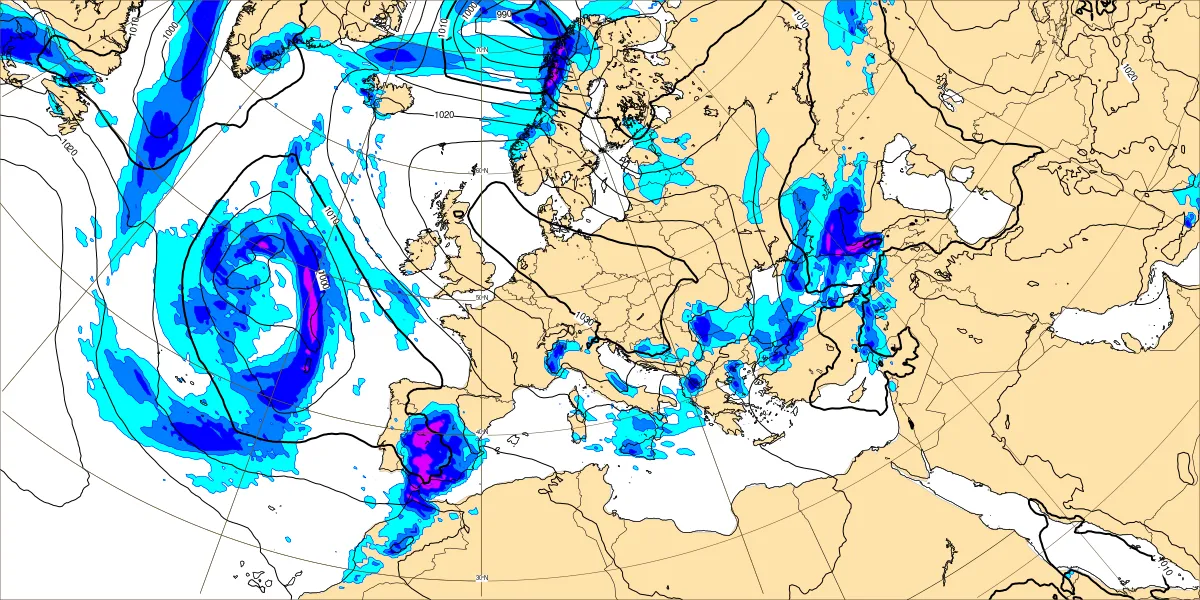
\includegraphics[width=\linewidth]{../Output/img_mapa_1.png}
      \par\vspace{2mm}
      \textbf{Mapa de isobaras a las 6:00 UTC}
  \end{minipage}
  \hfill
  \begin{minipage}{0.48\textwidth}
      \centering
      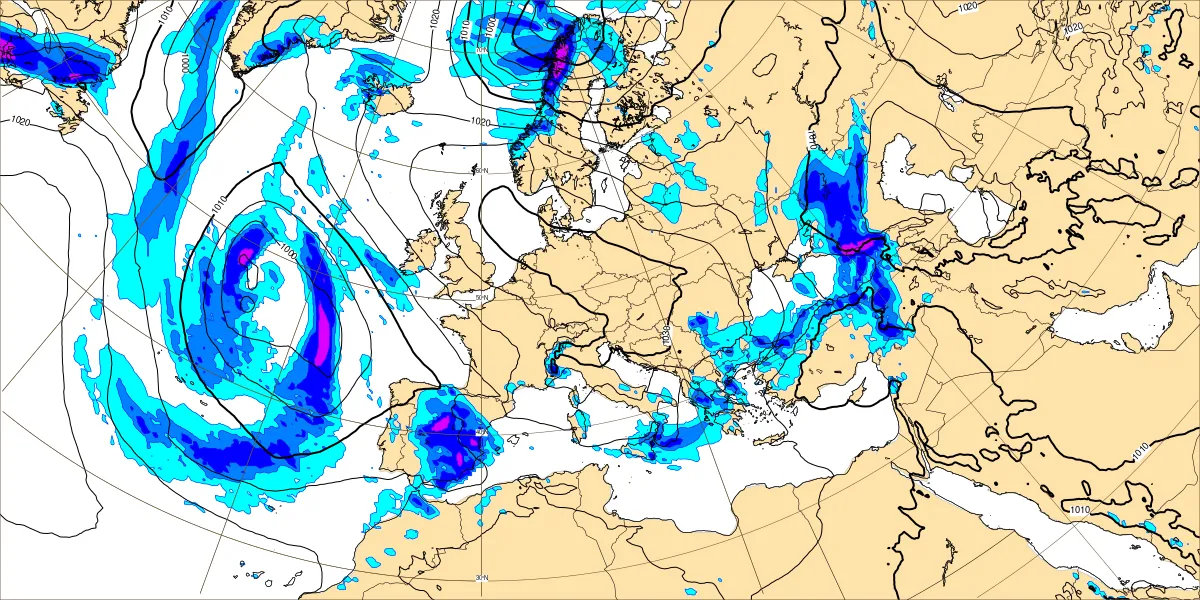
\includegraphics[width=\linewidth]{../Output/img_mapa_2.png}
      \par\vspace{2mm}
      \textbf{Imagen satélite a las 6:00 UTC}
  \end{minipage}

\end{textblock*}

\begin{textblock*}{3.9cm}(26.1cm, 2cm) 

  \resizebox{0.9\textwidth}{!}{%
  \renewcommand{\arraystretch}{1.2} 
  \setlength{\arrayrulewidth}{1.0pt} 
  
  \begin{tabular}{|c|l|}
  \hline
  \textbf{SS} & Estado de la mar \\
  \hline
  \textbf{W} & Viento \\
  \hline
  \textbf{P} & Precipitaciones \\
  \hline
  \textbf{V} & Visibilidad \\
  \hline
  \textbf{N} & Nocturnidad \\
  \hline
  \textbf{T} & Temperatura \\
  \hline
  \textbf{CC} & Techo de nubes \\
  \hline
  \end{tabular}
  }
  
  \end{textblock*}
  

\end{document} %Orden que finaliza el artículo, no puede haber nada escrito después de esta instrucción
